\begin{figure}[h]
\centering
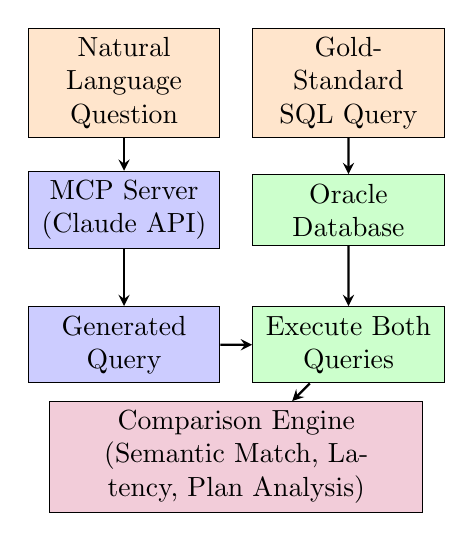
\begin{tikzpicture}[scale=0.95, node distance=1.5cm]
  \tikzstyle{block} = [rectangle, draw, fill=blue!20, text width=2.2cm, text centered, minimum height=0.8cm]
  \tikzstyle{io} = [rectangle, draw, fill=orange!20, text width=2.2cm, text centered, minimum height=0.8cm]
  \tikzstyle{process} = [rectangle, draw, fill=green!20, text width=2.2cm, text centered, minimum height=0.8cm]
  \tikzstyle{arrow} = [thick,->,>=stealth]

  % Layer 1: Input
  \node [io] (nl) at (0,2) {Natural Language\\Question};
  \node [io] (sql) at (3,2) {Gold-Standard\\SQL Query};

  % Layer 2: Processing
  \node [block] (mcp) at (0,0.3) {MCP Server\\(Claude API)};
  \node [process] (dbbase) at (3,0.3) {Oracle\\Database};
  
  % Layer 3: Execution
  \node [block] (mcpgen) at (0,-1.5) {Generated\\Query};
  \node [process] (exec) at (3,-1.5) {Execute Both\\Queries};
  
  % Layer 4: Comparison
  \node [rectangle, draw, fill=purple!20, text width=4.5cm, text centered, minimum height=0.8cm] (compare) at (1.5,-3)
    {Comparison Engine\\(Semantic Match, Latency, Plan Analysis)};

  % Arrows
  \draw [arrow] (nl) -- (mcp);
  \draw [arrow] (sql) -- (dbbase);
  \draw [arrow] (mcp) -- (mcpgen);
  \draw [arrow] (dbbase) -- (exec);
  \draw [arrow] (mcpgen) -- (exec);
  \draw [arrow] (exec) -- (compare);
  
\end{tikzpicture}
\caption{MCP Evaluation Pipeline Architecture. Natural language questions are simultaneously (1) sent to MCP server for SQL generation and (2) matched with gold-standard SQL. Both generated and baseline queries execute against Oracle Database. Results undergo semantic comparison, latency measurement, and query optimization analysis. Pipeline orchestrated by Python evaluation framework with 3-phase protocol.}
\label{fig:pipeline_architecture}
\end{figure}
